\let\negmedspace\undefined
\let\negthickspace\undefined
\documentclass[journal,12pt,twocolumn]{IEEEtran}
%\documentclass[conference]{IEEEtran}
%\IEEEoverridecommandlockouts
% The preceding line is only needed to identify funding in the first footnote. If that is unneeded, please comment it out.
\usepackage{cite}
\usepackage{amssymb,amsfonts,amsthm,amsmath}
\usepackage{algorithmic}
\usepackage{graphicx}
\usepackage{textcomp}
\usepackage{xcolor}
\usepackage{txfonts}
\usepackage{listings}
\usepackage{enumitem}
\usepackage{mathtools}
\usepackage{gensymb}

\usepackage{hyperref}
%%\usepackage{stmaryrd}
%%\usepackage{tkz-euclide} % loads  TikZ and tkz-base
%%\usetkzobj{all}
    \usepackage{color}                                            %%
    \usepackage{array}                                            %%
    \usepackage{longtable}                                        %%
    \usepackage{calc}                                             %%
    \usepackage{multirow}                                         %%
    \usepackage{hhline}                                           %%
    \usepackage{ifthen}                                           %%

\DeclareMathOperator*{\Res}{Res}
%\renewcommand{\baselinestretch}{2}
\renewcommand\thesection{\arabic{section}}
\renewcommand\thesubsection{\thesection.\arabic{subsection}}
\renewcommand\thesubsubsection{\thesubsection.\arabic{subsubsection}}

\renewcommand\thesectiondis{\arabic{section}}
\renewcommand\thesubsectiondis{\thesectiondis.\arabic{subsection}}
\renewcommand\thesubsubsectiondis{\thesubsectiondis.\arabic{subsubsection}}

% correct bad hyphenation here
\hyphenation{op-tical net-works semi-conduc-tor}
\def\inputGnumericTable{}                                 %%

\lstset{
language=tex,
frame=single, 
breaklines=true
}

\begin{document}
%


\newtheorem{theorem}{Theorem}[section]
\newtheorem{problem}{Problem}
\newtheorem{proposition}{Proposition}[section]
\newtheorem{lemma}{Lemma}[section]
\newtheorem{corollary}[theorem]{Corollary}
\newtheorem{example}{Example}[section]
\newtheorem{definition}[problem]{Definition}
%\newtheorem{thm}{Theorem}[section] 
%\newtheorem{defn}[thm]{Definition}
%\newtheorem{algorithm}{Algorithm}[section]
%\newtheorem{cor}{Corollary}
\newcommand{\BEQA}{\begin{eqnarray}}
\newcommand{\EEQA}{\end{eqnarray}}
\newcommand{\define}{\stackrel{\triangle}{=}}

\bibliographystyle{IEEEtran}
%\bibliographystyle{ieeetr}


\providecommand{\mbf}{\mathbf}
\providecommand{\pr}[1]{\ensuremath{\Pr\left(#1\right)}}
\providecommand{\re}[1]{\ensuremath{\text{Re}\left(#1\right)}}
\providecommand{\im}[1]{\ensuremath{\text{Im}\left(#1\right)}}
\providecommand{\qfunc}[1]{\ensuremath{Q\left(#1\right)}}
\providecommand{\sbrak}[1]{\ensuremath{{}\left[#1\right]}}
\providecommand{\lsbrak}[1]{\ensuremath{{}\left[#1\right.}}
\providecommand{\rsbrak}[1]{\ensuremath{{}\left.#1\right]}}
\providecommand{\brak}[1]{\ensuremath{\left(#1\right)}}
\providecommand{\lbrak}[1]{\ensuremath{\left(#1\right.}}
\providecommand{\rbrak}[1]{\ensuremath{\left.#1\right)}}
\providecommand{\cbrak}[1]{\ensuremath{\left\{#1\right\}}}
\providecommand{\lcbrak}[1]{\ensuremath{\left\{#1\right.}}
\providecommand{\rcbrak}[1]{\ensuremath{\left.#1\right\}}}
\theoremstyle{remark}
\newtheorem{rem}{Remark}
\newcommand{\sgn}{\mathop{\mathrm{sgn}}}
\providecommand{\abs}[1]{\left\vert#1\right\vert}
\providecommand{\res}[1]{\Res\displaylimits_{#1}} 
\providecommand{\norm}[1]{\left\lVert#1\right\rVert}
%\providecommand{\norm}[1]{\lVert#1\rVert}
\providecommand{\mtx}[1]{\mathbf{#1}}
\providecommand{\mean}[1]{E\left[ #1 \right]}
\providecommand{\fourier}{\overset{\mathcal{F}}{ \rightleftharpoons}}
%\providecommand{\hilbert}{\overset{\mathcal{H}}{ \rightleftharpoons}}
\providecommand{\system}{\overset{\mathcal{H}}{ \longleftrightarrow}}
	%\newcommand{\solution}[2]{\textbf{Solution:}{#1}}
\newcommand{\solution}{\noindent \textbf{Solution: }}
\providecommand{\dec}[2]{\ensuremath{\overset{#1}{\underset{#2}{\gtrless}}}}
\newcommand{\myvec}[1]{\ensuremath{\begin{pmatrix}#1\end{pmatrix}}}
\newcommand{\mydet}[1]{\ensuremath{\begin{vmatrix}#1\end{vmatrix}}}
	\newcommand*{\permcomb}[4][0mu]{{{}^{#3}\mkern#1#2_{#4}}}
\newcommand*{\perm}[1][-3mu]{\permcomb[#1]{P}}
\newcommand*{\comb}[1][-1mu]{\permcomb[#1]{C}}
\providecommand{\gauss}[2]{\mathcal{N}\ensuremath{\left(#1,#2\right)}}
%%
%	%\newcommand{\solution}[2]{\textbf{Solution:}{#1}}
%\newcommand{\solution}{\noindent \textbf{Solution: }}
\newcommand{\cosec}{\,\text{cosec}\,}
\newcommand{\sinc}{\,\text{sinc}\,}
\newcommand{\rect}{\,\text{rect}\,}

%\numberwithin{equation}{section}
\numberwithin{equation}{subsection}
%\numberwithin{problem}{section}
%\numberwithin{definition}{section}
\makeatletter
\@addtoreset{figure}{problem}
\makeatother

\let\StandardTheFigure\thefigure
\let\vec\mathbf
\let\j\jmath
%\renewcommand{\thefigure}{\theproblem.\arabic{figure}}
\renewcommand{\thefigure}{\theproblem}
%\setlist[enumerate,1]{before=\renewcommand\theequation{\theenumi.\arabic{equation}}
%\counterwithin{equation}{enumi}


%\renewcommand{\theequation}{\arabic{subsection}.\arabic{equation}}

\def\putbox#1#2#3{\makebox[0in][l]{\makebox[#1][l]{}\raisebox{\baselineskip}[0in][0in]{\raisebox{#2}[0in][0in]{#3}}}}
     \def\rightbox#1{\makebox[0in][r]{#1}}
     \def\centbox#1{\makebox[0in]{#1}}
     \def\topbox#1{\raisebox{-\baselineskip}[0in][0in]{#1}}
     \def\midbox#1{\raisebox{-0.5\baselineskip}[0in][0in]{#1}}

\vspace{3cm}

\title{
%	\logo{
	Probability: Assignment 2
%	}
}

\author{
	Sree Anusha Ganapathiraju\\
	CC22RESCH11003
	%<-this % stops a space
%\thanks{}}
}
\maketitle

\newpage

\tableofcontents

\bigskip

\renewcommand{\thefigure}{\theenumi}
\renewcommand{\thetable}{\theenumi}
%
		\numberwithin{equation}{enumi}
\section{Central Limit Theorem}
%
\begin{enumerate}[label=\thesection.\arabic*
,ref=\thesection.\theenumi]

%
\item
Generate $10^6$ samples of the random variable
%
\begin{equation}
X = \sum_{i=1}^{12}U_i -6
\end{equation}
%
using a C program, where $U_i, i = 1,2,\dots, 12$ are  a set of independent uniform random variables between 0 and 1
and save in a file called gau.dat\\
\solution 
\begin{lstlisting}
Assignment 2/codes/gxrand.c
Assignment 2/codes/coeffs.h
Assignment 2/codes/gau.dat
\end{lstlisting}
%
\item
Load gau.dat in python and plot the empirical CDF of $X$ using the samples in gau.dat. What properties does a CDF have?
\\
\solution The CDF of $X$ is plotted in Fig. \ref{fig:gauss_cdf}. The CDF defined for a continuous random variable is given as:\\
\begin{center}
$F_{X}(x)=\int_{-\infty}^{x}f_{X}(t)dt$
\end{center}
The cumulative distribution function $F_{X}(x)$ of a random variable has the following important properties:
\begin{itemize}
\item[1] Every CDF $F_{X}$ is non decreasing and right continuous i.e.,
$\lim_{x\to-\infty} F_{X}(x)=0$ and $\lim_{x\to\infty} F_{X}(x)=1$
\item[2] For all real numbers $a$ and $b$ with continuous random variable $X$, then the function $f_{x}$ is equal to the derivative of $F_{X}$, such that \\
$F_{X}(b)-F_{X}(a)=P(a<x<b)=\int_{a}^{b}f_{X}(x)dx$
\item[3] If $X$ is a completely discrete random variable, then it takes the values $x_1$, $x_2$, $x_3$,..  with probability $p_i = p(x_i)$, and the CDF of $X$ will be discontinuous at the points $x_i$:\\
$F_{X}(x)=P(X\leq x)=\sum_{x_i\leq x}P(X=x_i)=\sum_{x_i-x\leq x}p(x_i)$
\\
\end{itemize}
\begin{figure}
\centering
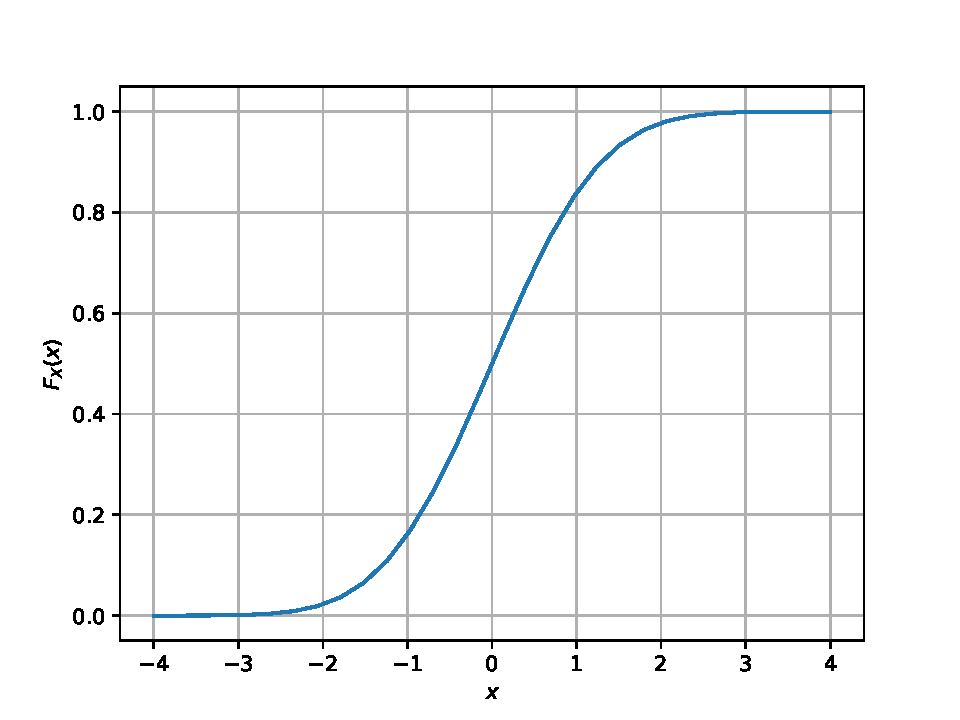
\includegraphics[width=\columnwidth]{./figs/gauss_cdf}
\caption{The CDF of $X$}
\label{fig:gauss_cdf}
\end{figure}
\item
Load gau.dat in python and plot the empirical PDF of $X$ using the samples in gau.dat. The PDF of $X$ is defined as
\begin{align}
p_{X}(x) = \frac{d}{dx}F_{X}(x)
\end{align}
What properties does the PDF have?
\\
\solution The PDF of $X$ is plotted in Fig. \ref{fig:gauss_pdf} using the code below.
\begin{lstlisting}
Assignment 2/codes/pdf_plot.py
\end{lstlisting}
The PDF is given by \\
\begin{center}
$P(a\leq x\leq b)=\int_{a}^{b}f(x)dx$
\end{center}
Let $X$ be the continuous random variable with density function $f(X)$, and the probability density function should satisfy the following conditions:
\begin{itemize}
\item[1] For a continuous random variable that takes some value between certain limits, say $a$ and $b$, the PDF is calculated by finding the area under its curve and the $X$-axis within the lower limit $(a)$ and upper limit $(b)$. Thus, the PDF is given by $\int_{a}^{b} f(x)dx$.

\item[2] The probability density function is non-negative for all the possible values, i.e. $f(x)\geq 0$, for all $x$.

\item[3] The area between the density curve and horizontal $X$-axis is equal to $1$, i.e.\\$\int_{-\infty}^{\infty}f(x)dx=1$

\item[4] Due to the property of continuous random variables, the density function curve is continued for all over the given range. Also, this defines itself over a range of continuous values or the domain of the variable.
\end{itemize}
\begin{figure}
\centering
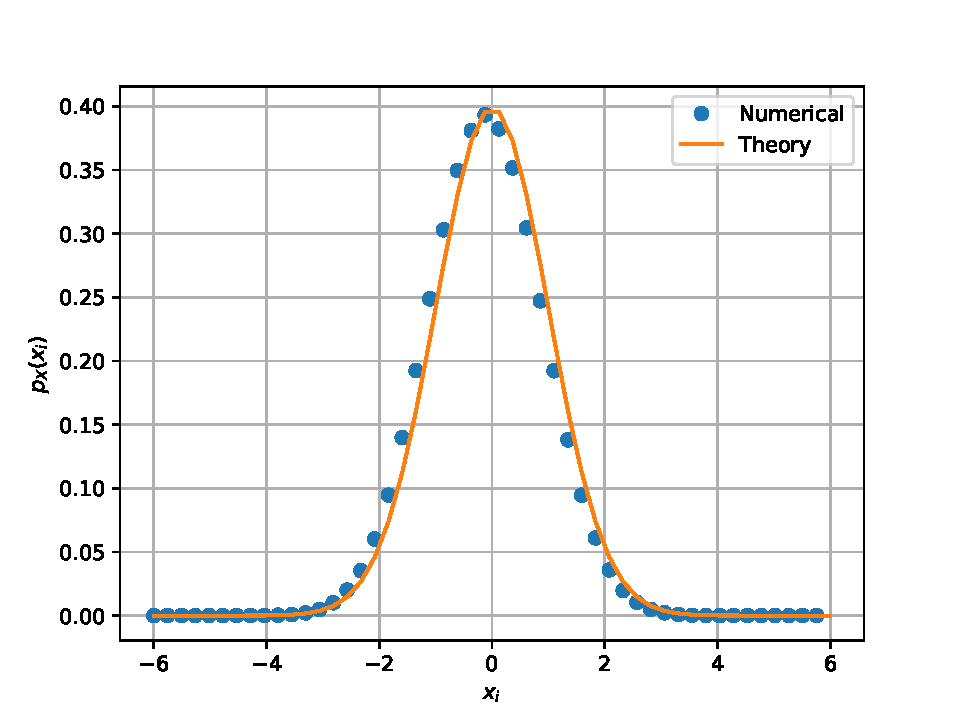
\includegraphics[width=\columnwidth]{./figs/gauss_pdf}
\caption{The PDF of $X$}
\label{fig:gauss_pdf}
\end{figure}
\item Find the mean and variance of $X$ by writing a C program.\\
\solution
\begin{lstlisting}
Assignment 2/codes/gxrand.c
\end{lstlisting}
The value of mean is 0.000 and variance Value: 1.000.
\item Given that 
\begin{align}
p_{X}(x) = \frac{1}{\sqrt{2\pi}}\exp\brak{-\frac{x^2}{2}}, -\infty < x < \infty,
\end{align}
repeat the above exercise theoretically.\\
\solution
The expected value (Mean) for standard normal distribution is $X$ is derived as:
\begin{align*}
& E[X]= \int_{-\infty}^{\infty}xf_{X}(x)dx
\\
& =\frac{1}{\sqrt{2\pi}}\int_{-\infty}^{\infty}x\exp\left(\frac{-x^2}{2}\right)dx
\\
& =\frac{1}{\sqrt{2\pi}}\int_{-\infty}^{0} x\exp\left(\frac{-x^2}{2}\right)dx + \frac{1}{\sqrt{2\pi}}\int_{0}^{\infty} x\exp\left(\frac{-x^2}{2}\right)dx
\\
& =\frac{1}{\sqrt{2\pi}}\left(\frac{-x^2}{2}\right)_{-\infty}^{0}+ \frac{1}{\sqrt{2\pi}}\left(\frac{-x^2}{2}\right)_{0}^{\infty}
\\
& =\frac{1}{\sqrt{2\pi}}[-1+0]+\frac{1}{\sqrt{2\pi}}[0+1]
\\
& =\frac{1}{\sqrt{2\pi}}-\frac{1}{\sqrt{2\pi}}
\\
& =0
\end{align*}
The variance can be calculated by
$Var[X]=E[X^2]-E[X]^2$\\
So we have,
\begin{align*}
& E[X^2]=\int_{-\infty}^{\infty}x^2 f_{X}(x)dx
\\ 
& =\frac{1}{\sqrt{2\pi}}\int_{-\infty}^{\infty}x^2\exp\left(\frac{-x^2}{2}\right)dx
\\
& =\left[\frac{1}{\sqrt{2\pi}}\int_{-\infty}^{0}x^2\exp\left(\frac{-x^2}{2}\right)dx\right]+\left]\frac{1}{\sqrt{2\pi}}\int_{0}^{\infty}x^2\exp\left(\frac{-x^2}{2}\right)dx\right]
\end{align*}
Upon integrating by parts the first part and second part in the above equation, we get 
\begin{align*}
&=\frac{1}{\sqrt{2\pi}}\Biggl\{\left[-x\exp\left(\frac{-x^2}{2}\right)\right]_{-\infty}^{0}+\int_{-\infty}^{0}\exp\left(\frac{-x^2}{2}\right)dx\Biggr\}+\frac{1}{\sqrt{2\pi}}\Biggl\{\left[-x\exp\left(\frac{-x^2}{2}\right)\right]_0^{\infty}+
 \frac{1}{\sqrt{2\pi}}\int_{0}^{\infty}\exp\left(\frac{-x^2}{2}\right)dx\Biggr\}
\\ 
&=\frac{1}{\sqrt{2\pi}}\Biggl\{(0-0)+\int_{-\infty}^{0}\exp\left(\frac{-x^2}{2}\right)dx+(0-0)+\int_{0}^{\infty}\exp\left(\frac{-x^2}{2}\right)dx   \Biggr\}
\\
&=\frac{1}{\sqrt{2\pi}}\int_{-\infty}^{\infty}\exp\left(\frac{-x^2}{2}\right)dx
\\
&\text{The probability density fucntion over the entire region is 1}
\\
&=\frac{1}{\sqrt{2\pi}}\int_{-\infty}^{\infty}\exp\left(\frac{-x^2}{2}\right)dx
\\
& =1
\end{align*}
From above, we know that \\
$E[X]^2=0^2=0$\\
$\text{Var}[X]=E[X^2]-E[X]^2=1-0=1$\\
Hence Proved.



\end{enumerate}
\end{document}
